  % this file is called up by thesis.tex
% content in this file will be fed into the main document
% ----------------------- name of chapter  -------------------------
\newgeometry{top=-0.1cm, left=1.2cm, right=1.5cm, bottom=1.45cm}
\chapter{Background only fit in CRs}
\label{app:stat:tzc:bonly:cr}
% ----------------------- paths to graphics ------------------------

% change according to folder and file names
\ifpdf
\graphicspath{Chapters/CH7/figures/BONLY_CR_UsingDL1rcFullSys}
\else
\graphicspath{Chapters/CH7/figures/BONLY_CR_UsingDL1rcFullSys}
\fi
\vspace{-1cm}

To check the background modeling and extract realistic background
normalisations, a CRs-only background-only fit using real data in CRs
is performed. \\
A summary of plots shown in the following:
\begin{itemize}
\item The value of the post-fit normalisation parameters of the free
floating background is shown in \cref{fig:stat:tzc:bonly:cr:norm}.
\item The list of the systematic shapes that are dropped from the fit for
each sample and for each region is shown in \Cref{fig:stat:tzc:bonly:cr:pruning}.
\item The pull distributions of the all nuisance parameters can be seen in
\Cref{fig:stat:tzc:bonly:cr:np:instr,fig:stat:tzc:bonly:cr:np:model} and \Cref{fig:stat:tzc:bonly:cr:gamma}. 
\item Event yields pre- and post-fit are shown in \Cref{tab:stat:tzc:bonly:cr:yields:prefit,tab:stat:tzc:bonly:cr:yields:postfit}. 
\item Pre-fit and post-fit distributions of the fitted distributions in the
various regions are shown in \Cref{fig:stat:tzc:bonly:cr:crplots:1,fig:stat:tzc:bonly:cr:crplots:2}.
\end{itemize}
As shown in \cref{fig:stat:tzc:bonly:cr:norm}, the \ttbar scale factor
is \SI{0.93\pm0.25}{}, compatible with unity. The pull distributions show that the \VVHF
normalisation is pulled up (\cref{fig:stat:tzc:bonly:cr:np:model}), 
driven by the prediction being lower than data in the side-band CRs
(\cref{tab:stat:tzc:bonly:cr:yields:prefit,tab:stat:tzc:bonly:cr:yields:postfit}).  
Since this fit uses real data in CRs, some pulls and constraints of
the NPs are expected. For the NPs for the instrumental uncertainties,
no significant pulls nor constraints are present (\cref{fig:stat:tzc:bonly:cr:np:instr}), 
while some NPs for the modeling uncertainties can be seen
(\cref{fig:stat:tzc:bonly:cr:np:model}), in particular for the \ttbar
and diboson backgrounds. 
After the fit, there is an overall good agreement between data and the
prediction, as it can be seen in the post-fit event yields
(\cref{tab:stat:tzc:bonly:cr:yields:postfit}) and in the distribution
of the fitted variables in the CRs
(\cref{fig:stat:tzc:bonly:cr:crplots:1,fig:stat:tzc:bonly:cr:crplots:2}). 

\begin{figure}[!htbp]
	\centering
	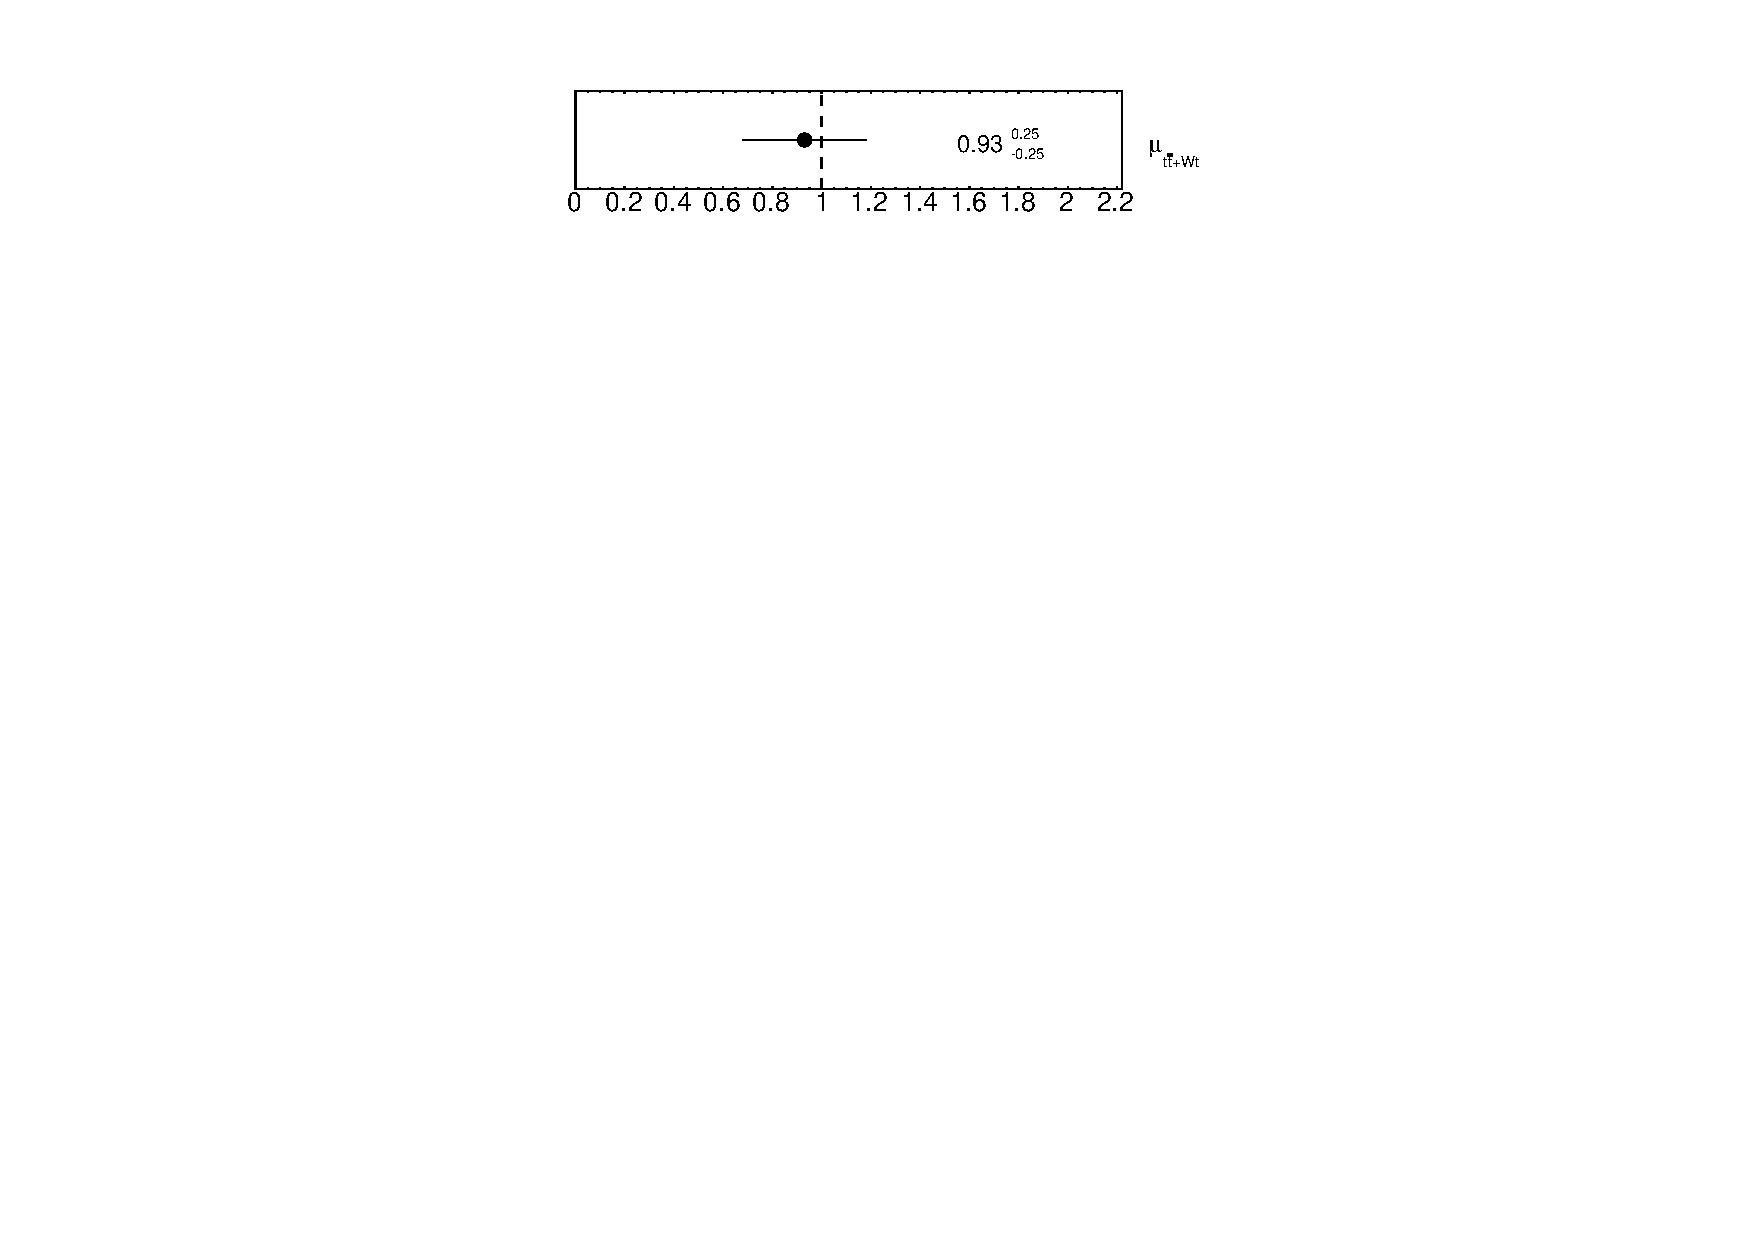
\includegraphics[width=.56\textwidth]{Chapters/CH7/figures/BONLY_CR_UsingDL1rcFullSys/NormFactors}
	\caption{Normalisation factors for the B-only \tZc fit in CRs.}%
	\label{fig:stat:tzc:bonly:cr:norm}
\end{figure}

\restoregeometry

\begin{figure}[htbp]
	\centering
	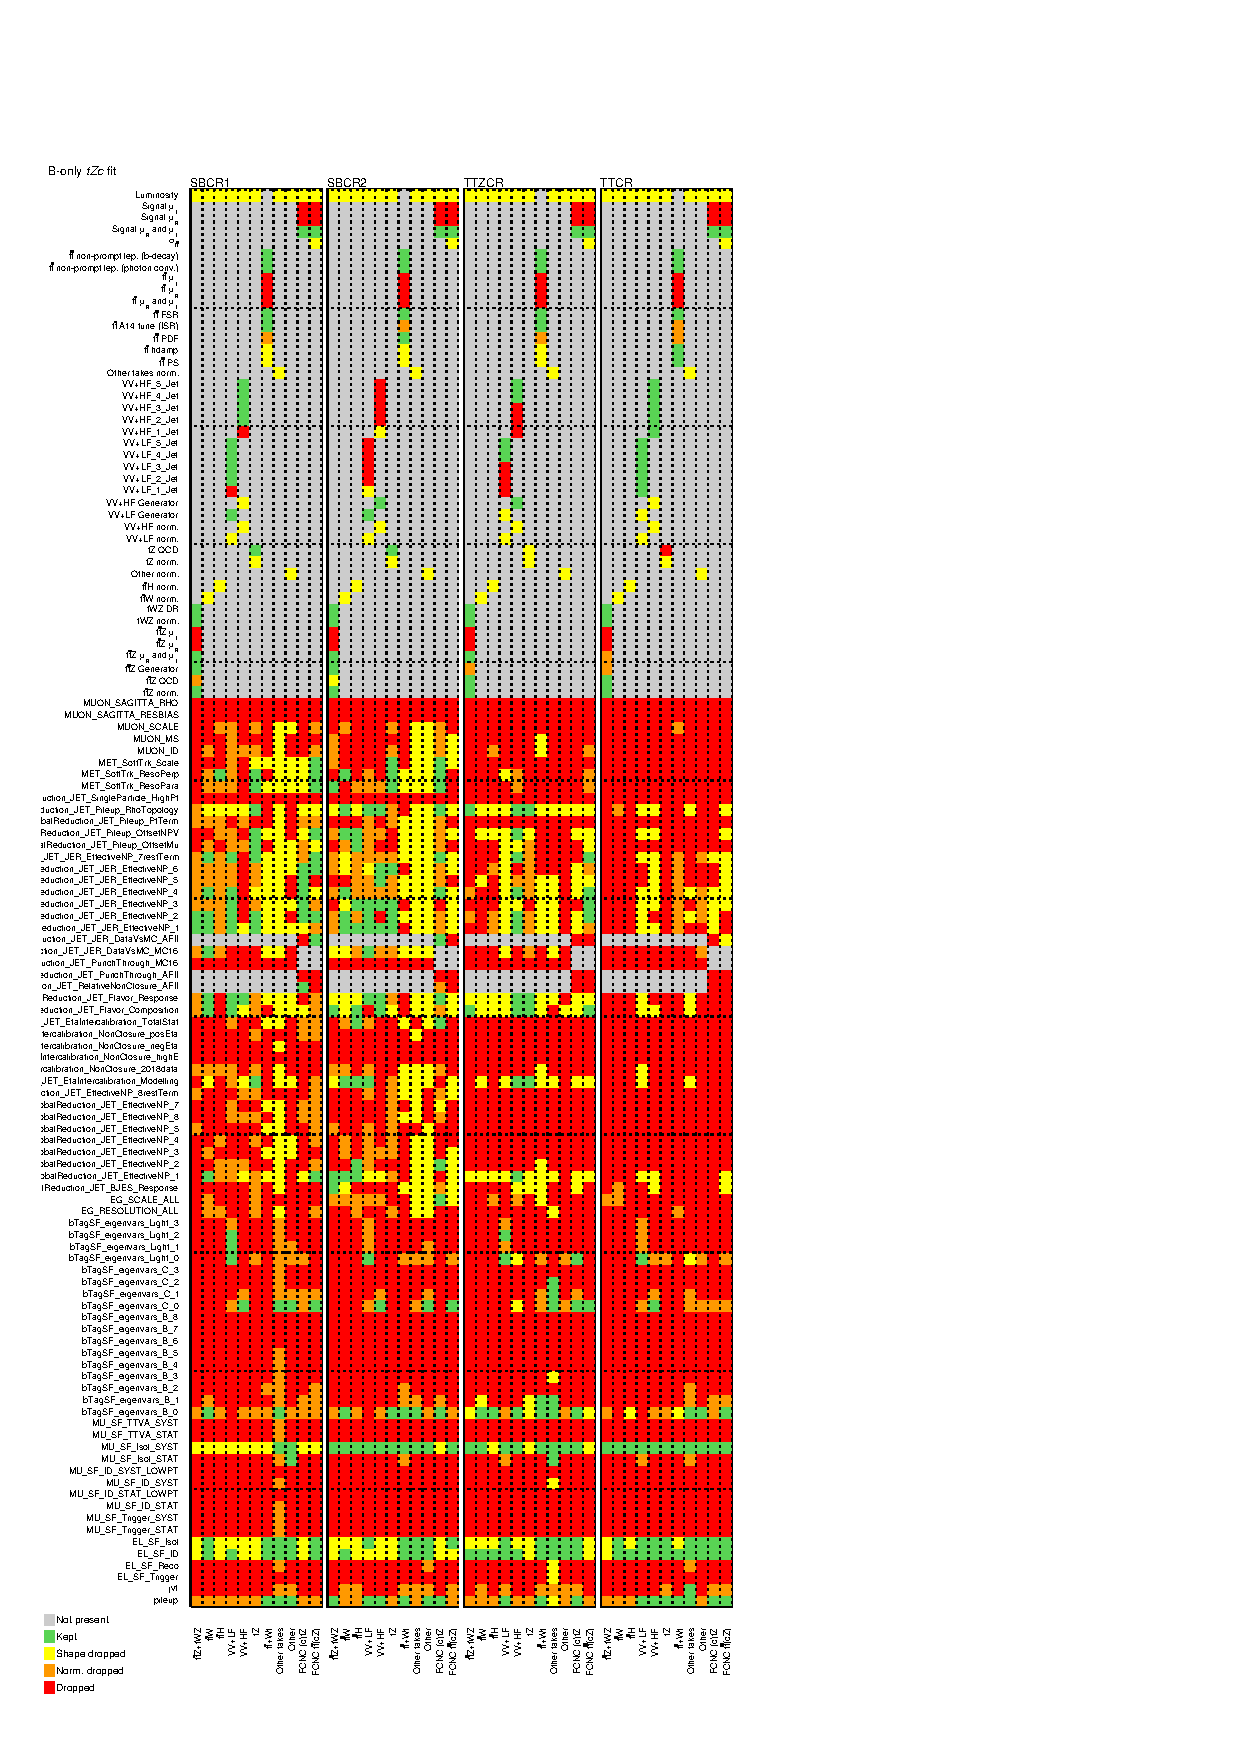
\includegraphics[width=.65\textwidth]{Chapters/CH7/figures/BONLY_CR_UsingDL1rcFullSys/Pruning}
	\caption{Pruning of the nuisance parameters for the B-only \tZc fit in CRs.}%
	\label{fig:stat:tzc:bonly:cr:pruning}
\end{figure}

\begin{figure}[htbp]
	\centering
	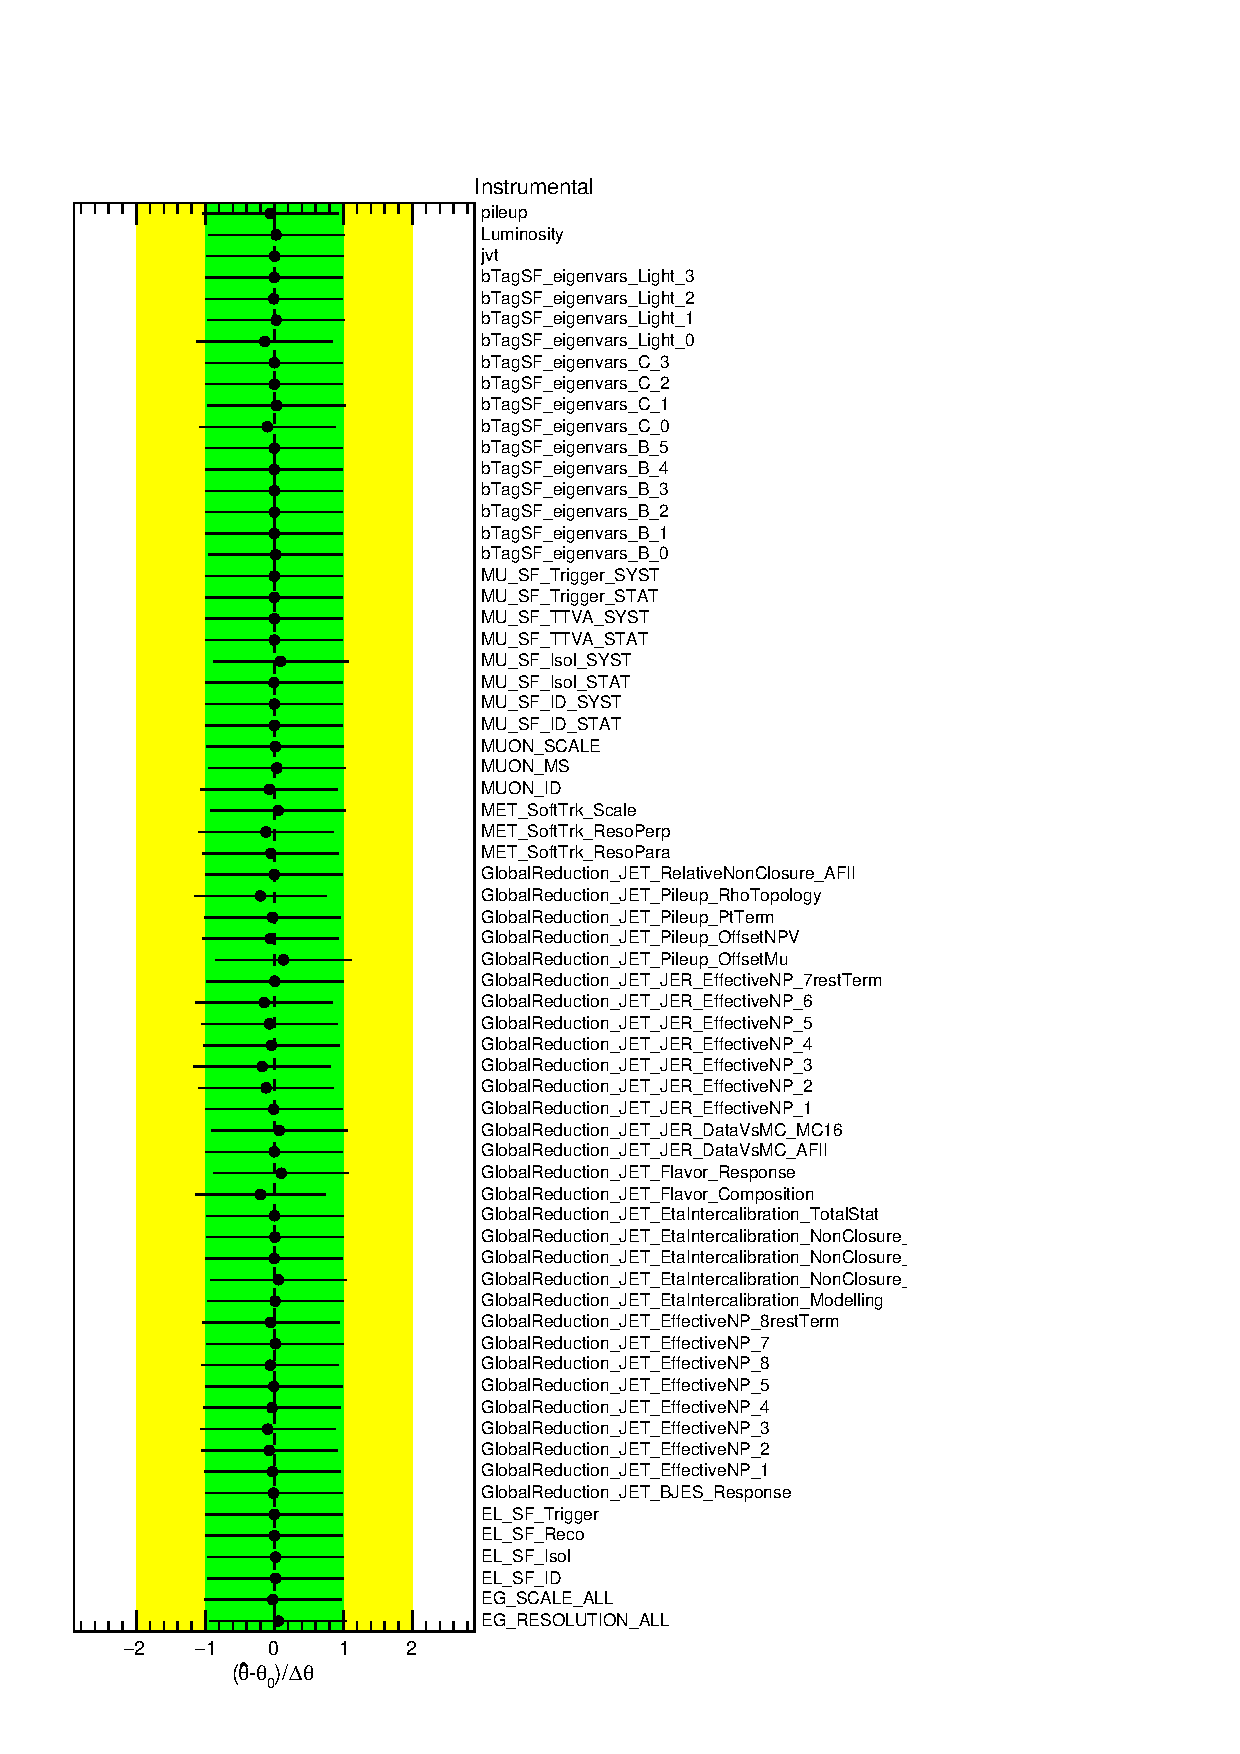
\includegraphics[width=.8\textwidth]{Chapters/CH7/figures/BONLY_CR_UsingDL1rcFullSys/NuisPar_Instrumental}
	\caption{Pulls and constraints of the instrumental nuisance parameters for the B-only \tZc fit in CRs.}%
	\label{fig:stat:tzc:bonly:cr:np:instr}
\end{figure}

\begin{figure}[htbp]
	\centering
	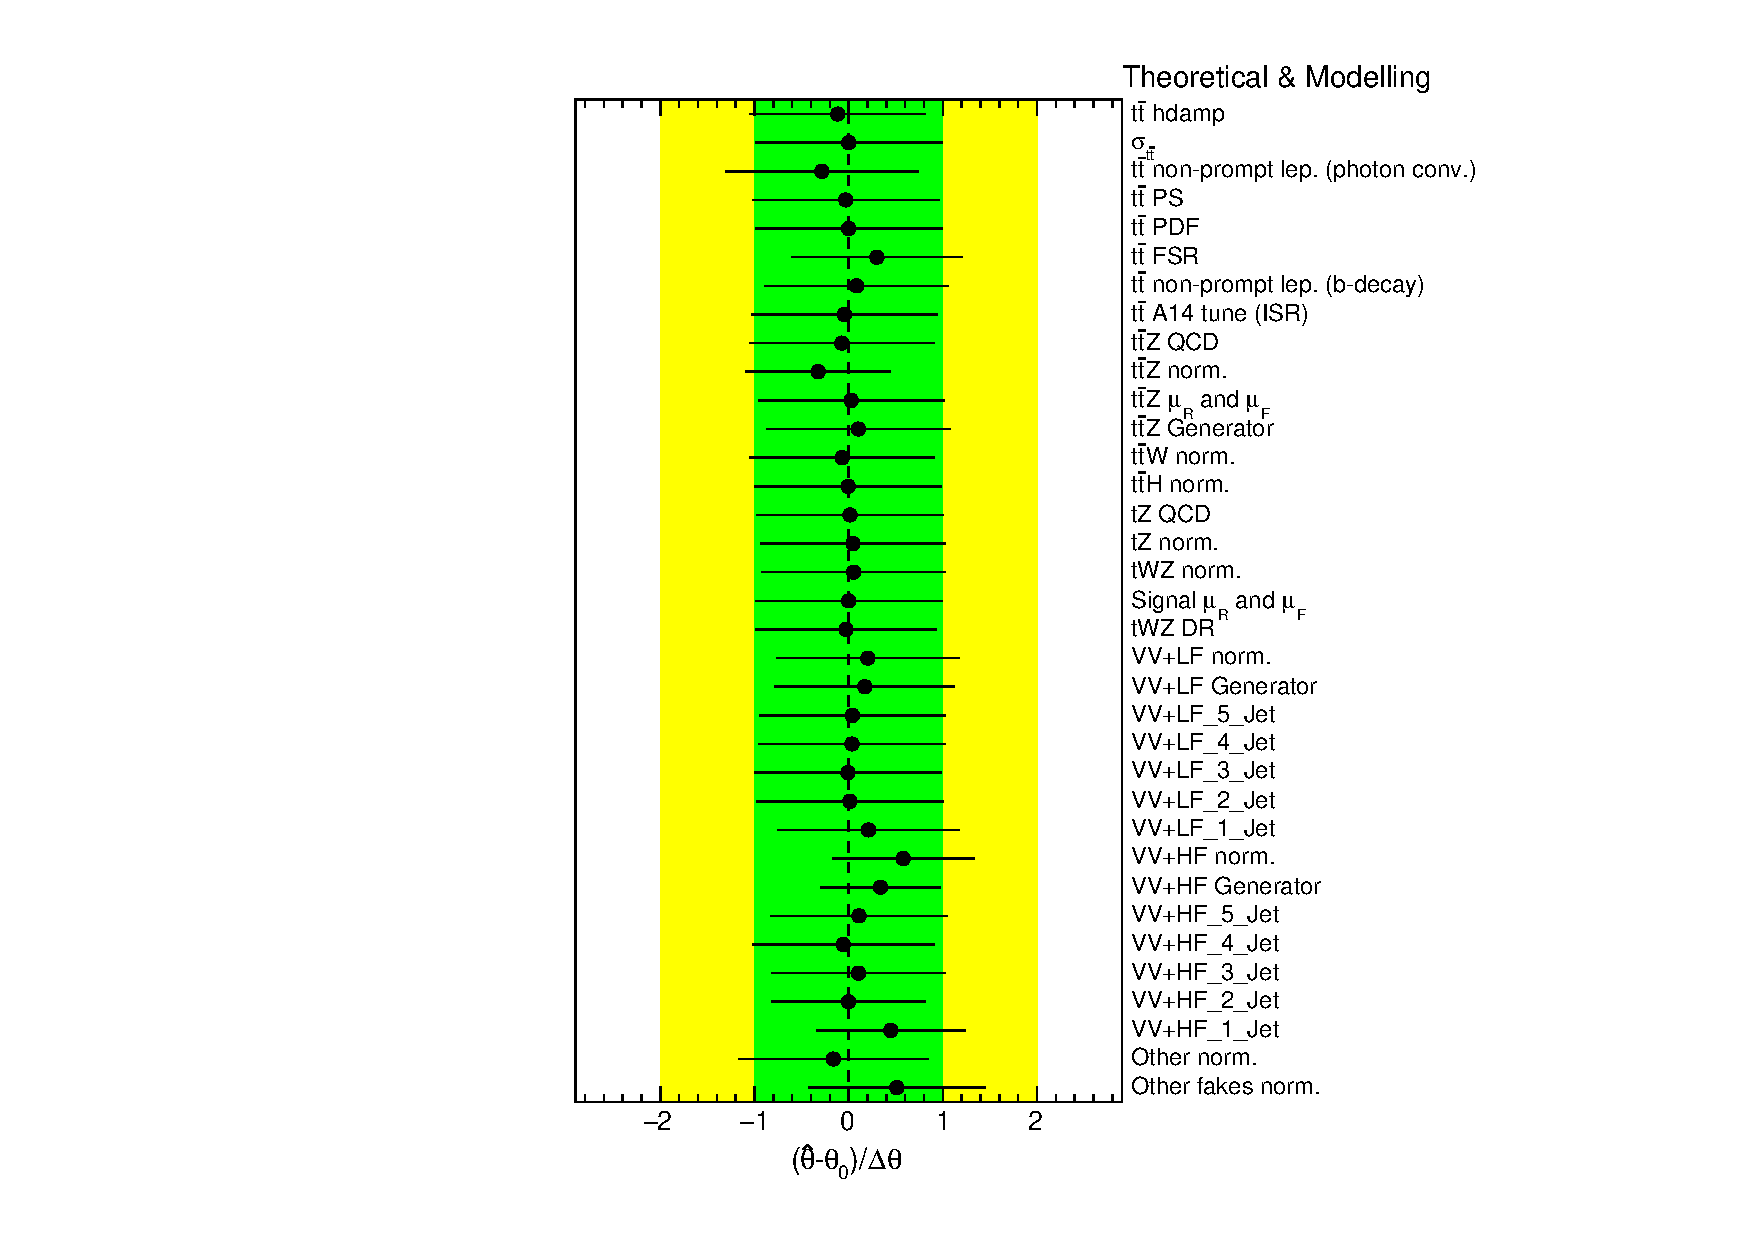
\includegraphics[width=.85\textwidth]{Chapters/CH7/figures/BONLY_CR_UsingDL1rcFullSys/NuisPar_Theoretical_&_Modelling}
	\caption{Pulls and constraints of the theoretical and modeling nuisance parameters for the B-only \tZc fit in CRs.}%
	\label{fig:stat:tzc:bonly:cr:np:model}
\end{figure}

\begin{figure}[htbp]
	\centering
	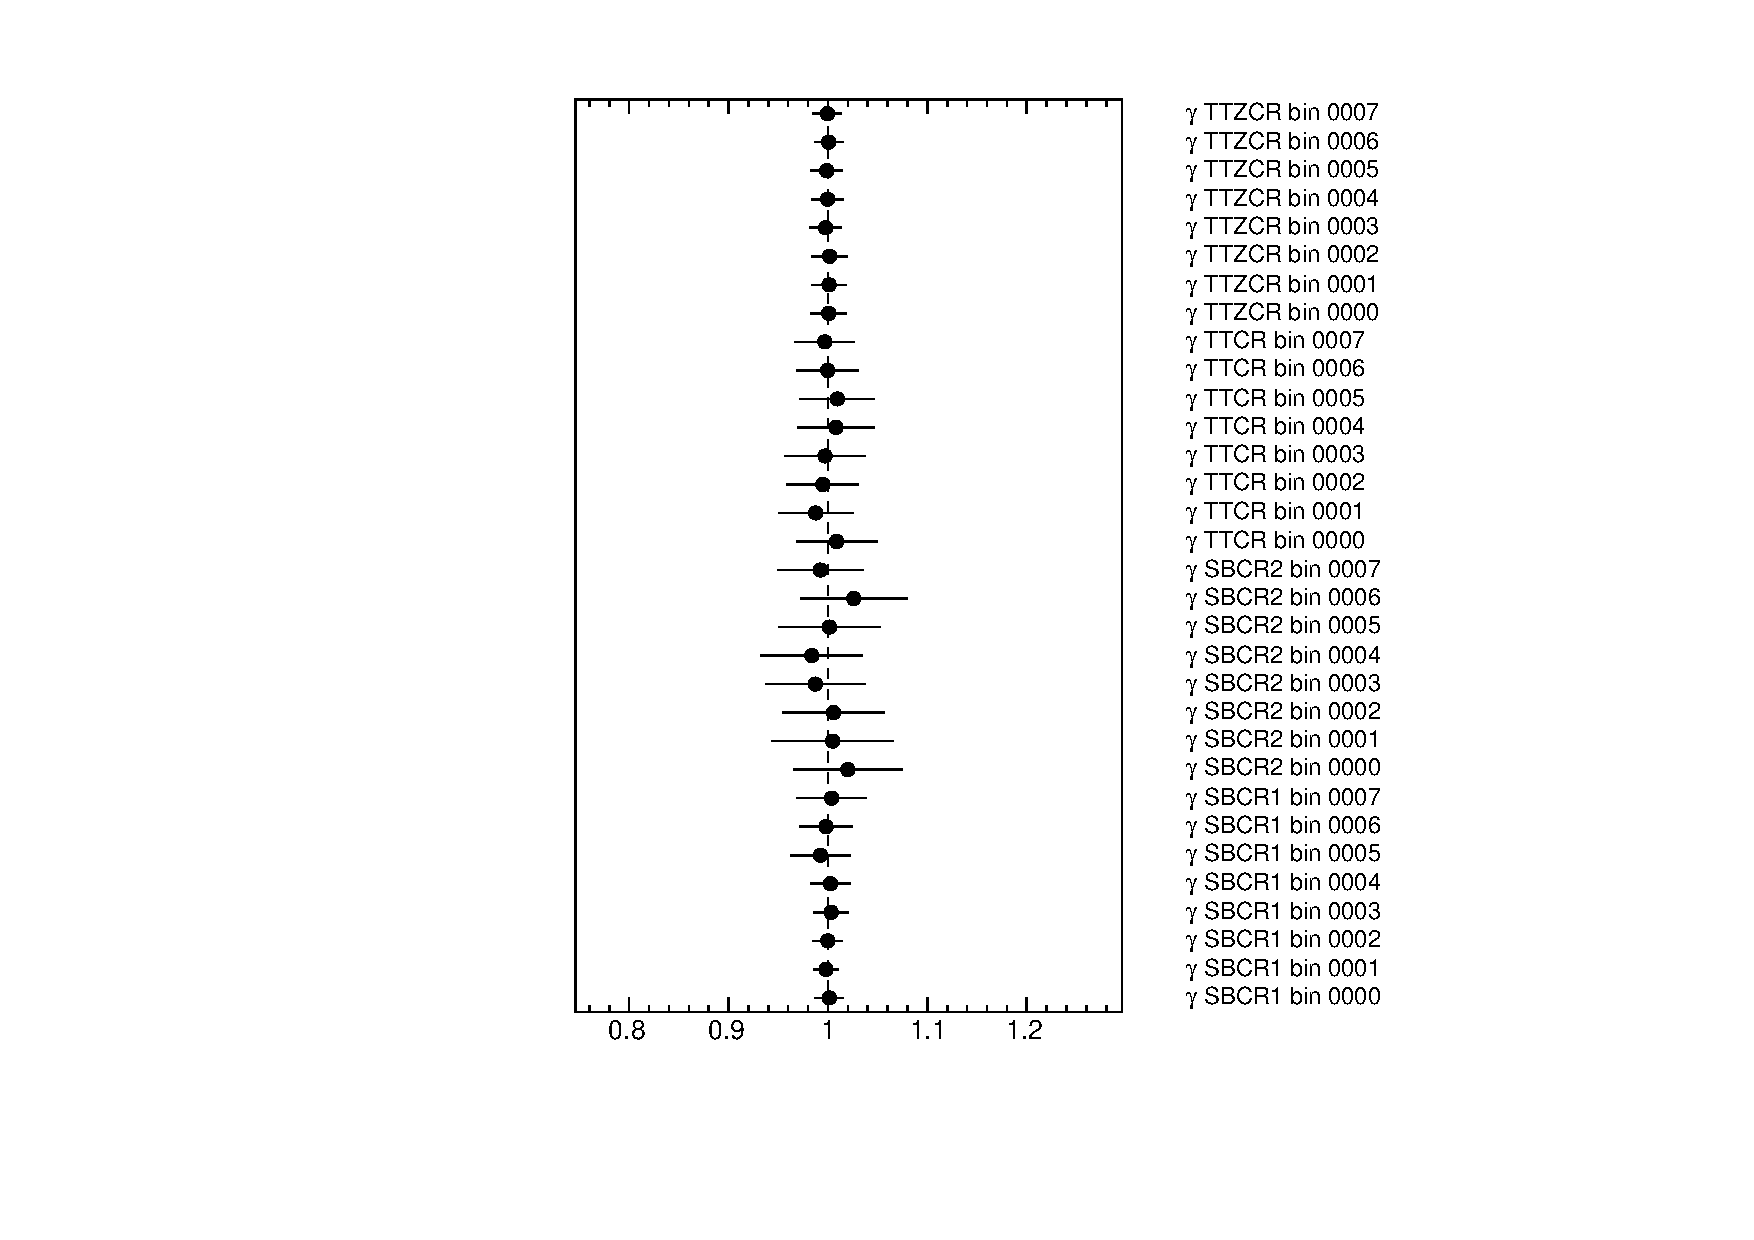
\includegraphics[width=.85\textwidth]{Chapters/CH7/figures/BONLY_CR_UsingDL1rcFullSys/Gammas}
	\caption{Gamma parameters for the B-only \tZc fit in CRs.}%
	\label{fig:stat:tzc:bonly:cr:gamma}
\end{figure}

\FloatBarrier

\begin{table}[]
	\footnotesize
	\centering
	% NB: add to main document: 
% \usepackage{siunitx} 
% \sisetup{separate-uncertainty,table-format=6.3(6)}  % hint: modify table-format to best fit your tables
\begin{tabular}{|p{0.16\textwidth}|>{\centering}p{0.16\textwidth}|>{\centering}p{0.16\textwidth}|>{\centering}p{0.16\textwidth}|>{\centering\arraybackslash}p{0.16\textwidth}|}
\toprule  
 & {Side-band CR1} & {Side-band CR2} & {\ttZ CR} & {\ttbar CR}\\
\midrule 
 \ttZ+\tWZ   & 88 $\pm$ 12 & 9.1 $\pm$ 2.1 & 164 $\pm$ 22 & 14.8 $\pm$ 1.9 \\ 
\ttW   & 4.3 $\pm$ 0.7 & 2.5 $\pm$ 0.5 & 2.3 $\pm$ 0.5 & 27 $\pm$ 4 \\ 
\ttH   & 2.3 $\pm$ 0.4 & 0.36 $\pm$ 0.07 & 5.4 $\pm$ 0.9 & 13.8 $\pm$ 2.1 \\ 
\VVLF   & 25 $\pm$ 15 & 18 $\pm$ 7 & 0.20 $\pm$ 0.22 & 0.40 $\pm$ 0.21 \\ 
\VVHF   & 130 $\pm$ 80 & 69 $\pm$ 28 & 13 $\pm$ 11 & 2.3 $\pm$ 1.4 \\ 
\tZq   & 20 $\pm$ 4 & 9.9 $\pm$ 1.7 & 14.6 $\pm$ 2.9 & 0.90 $\pm$ 0.15 \\ 
\ttbar+Wt   & 10 $\pm$ 4 & 9.1 $\pm$ 2.7 & 3.0 $\pm$ 1.2 & 102 $\pm$ 24 \\ 
Other fakes   & 3 $\pm$ 5 & 10 $\pm$ 11 & 0.00 $\pm$ 0.06 & 0.12 $\pm$ 0.14 \\ 
Other   & 2.2 $\pm$ 1.6 & 0.8 $\pm$ 2.6 & 1.1 $\pm$ 0.5 & 2.9 $\pm$ 1.5 \\ 
\midrule 
Total background  & 280 $\pm$ 80 & 130 $\pm$ 32 & 203 $\pm$ 27 & 164 $\pm$ 25 \\ 
\midrule 
Data   & 331 & 169 & 197 & 156 \\ 
\midrule 
Data / Bkg.   & 1.18 $\pm$ 0.35 & 1.30 $\pm$ 0.34 & 0.97 $\pm$ 0.14 & 0.95 $\pm$ 0.16 \\ 
\bottomrule 
\end{tabular} 

	\caption{Pre-fit event yields in the CRs for the B-only fit for the \tZc coupling extraction. \TabErrStatSys} 
	\label{tab:stat:tzc:bonly:cr:yields:prefit}
\end{table} 
\begin{table}[]
	\footnotesize
	\centering
	% NB: add to main document: 
% \usepackage{siunitx} 
% \sisetup{separate-uncertainty,table-format=6.3(6)}  % hint: modify table-format to best fit your tables
\begin{tabular}{|l|S|S|S|S|}
\toprule  
 & {Side-band CR1tZc} & {Side-band CR2} & {\ttZ CR} & {\ttbar CR}\\
\midrule 
  \ttZ+\tWZ   & 86 \pm 10 & 9.3 \pm 2.1 & 157 \pm 13 & 14.4 \pm 1.4 \\ 
  \ttW   & 4.2 \pm 0.7 & 2.5 \pm 0.5 & 2.2 \pm 0.4 & 26 \pm 4 \\ 
  \ttH   & 2.3 \pm 0.4 & 0.37 \pm 0.07 & 5.3 \pm 0.8 & 13.8 \pm 2.1 \\ 
  \VVLF   & 29 \pm 16 & 21 \pm 8 & 0.23 \pm 0.23 & 0.40 \pm 0.19 \\ 
  \VVHF   & 172 \pm 28 & 94 \pm 18 & 18 \pm 7 & 3.3 \pm 0.6 \\ 
  \tZq   & 20 \pm 4 & 10.1 \pm 1.7 & 14.4 \pm 2.7 & 0.91 \pm 0.13 \\ 
  \ttbar+Wt   & 9.4 \pm 2.9 & 8.6 \pm 1.7 & 2.5 \pm 0.8 & 95 \pm 13 \\ 
  Other fakes   & 5 \pm 5 & 18 \pm 16 & 0.006 \pm 0.009 & 0.18 \pm 0.15 \\ 
  Other   & 1.8 \pm 1.2 & 0.3 \pm 0.9 & 1.0 \pm 0.5 & 2.7 \pm 1.4 \\ 
\midrule 
  Total background  & 329 \pm 20 & 165 \pm 14 & 201 \pm 13 & 157 \pm 12 \\ 
\midrule 
  Data   & 331 & 169 & 197 & 156 \\ 
\midrule 
  Data / Bkg.   & 1.01 \pm 0.06 & 1.02 \pm 0.09 & 0.98 \pm 0.06 & 0.99 \pm 0.08 \\ 
\bottomrule 
\end{tabular} 

	\caption{Post-fit event yields in the CRs for the B-only fit for the \tZc coupling extraction. \TabErrStatSys} 
	\label{tab:stat:tzc:bonly:cr:yields:postfit}
\end{table} 

\FloatBarrier

\begin{figure}[htbp]
	\centering
	\begin{tabular}{cc}
		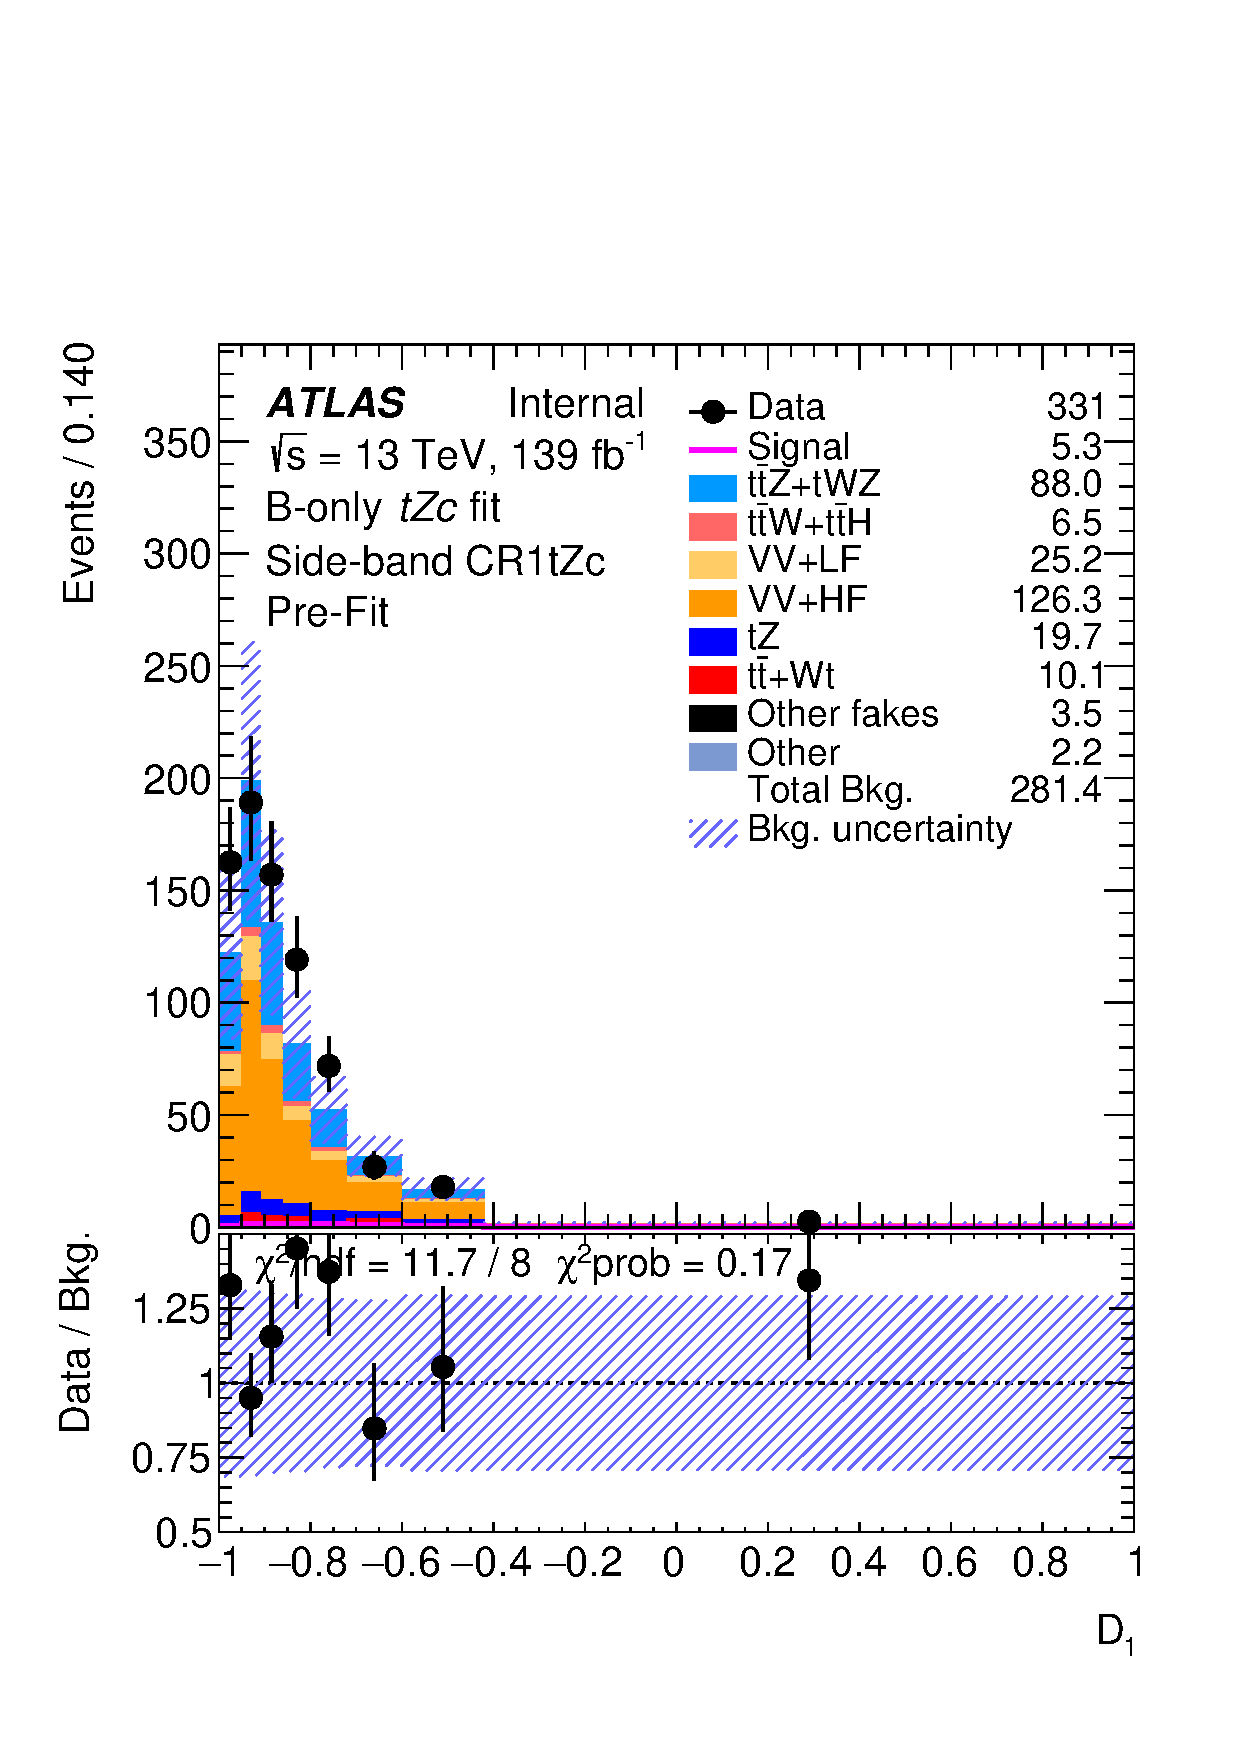
\includegraphics[width=.45\textwidth]{Chapters/CH7/figures/BONLY_CR_UsingDL1rcFullSys/Plots/SBCR1} &
		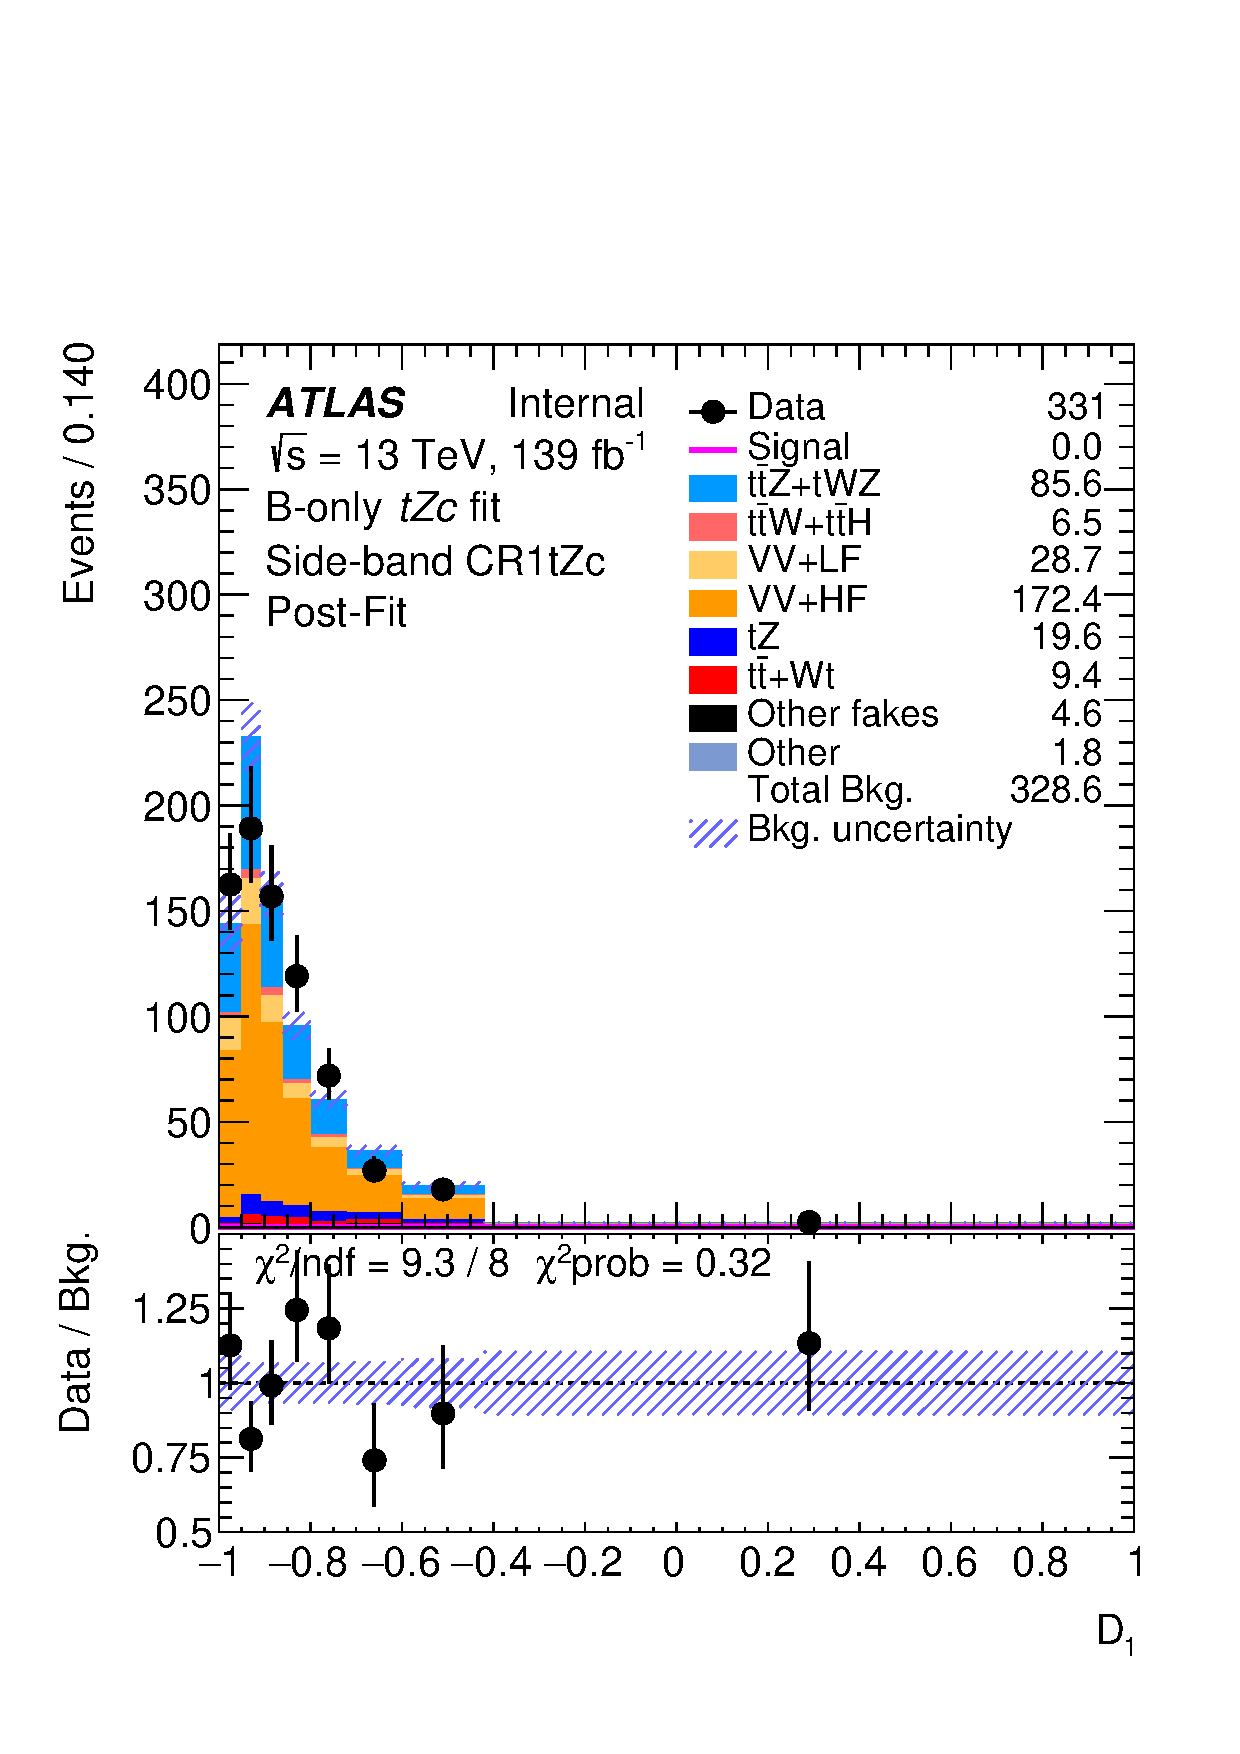
\includegraphics[width=.45\textwidth]{Chapters/CH7/figures/BONLY_CR_UsingDL1rcFullSys/Plots/SBCR1_postFit} \\
		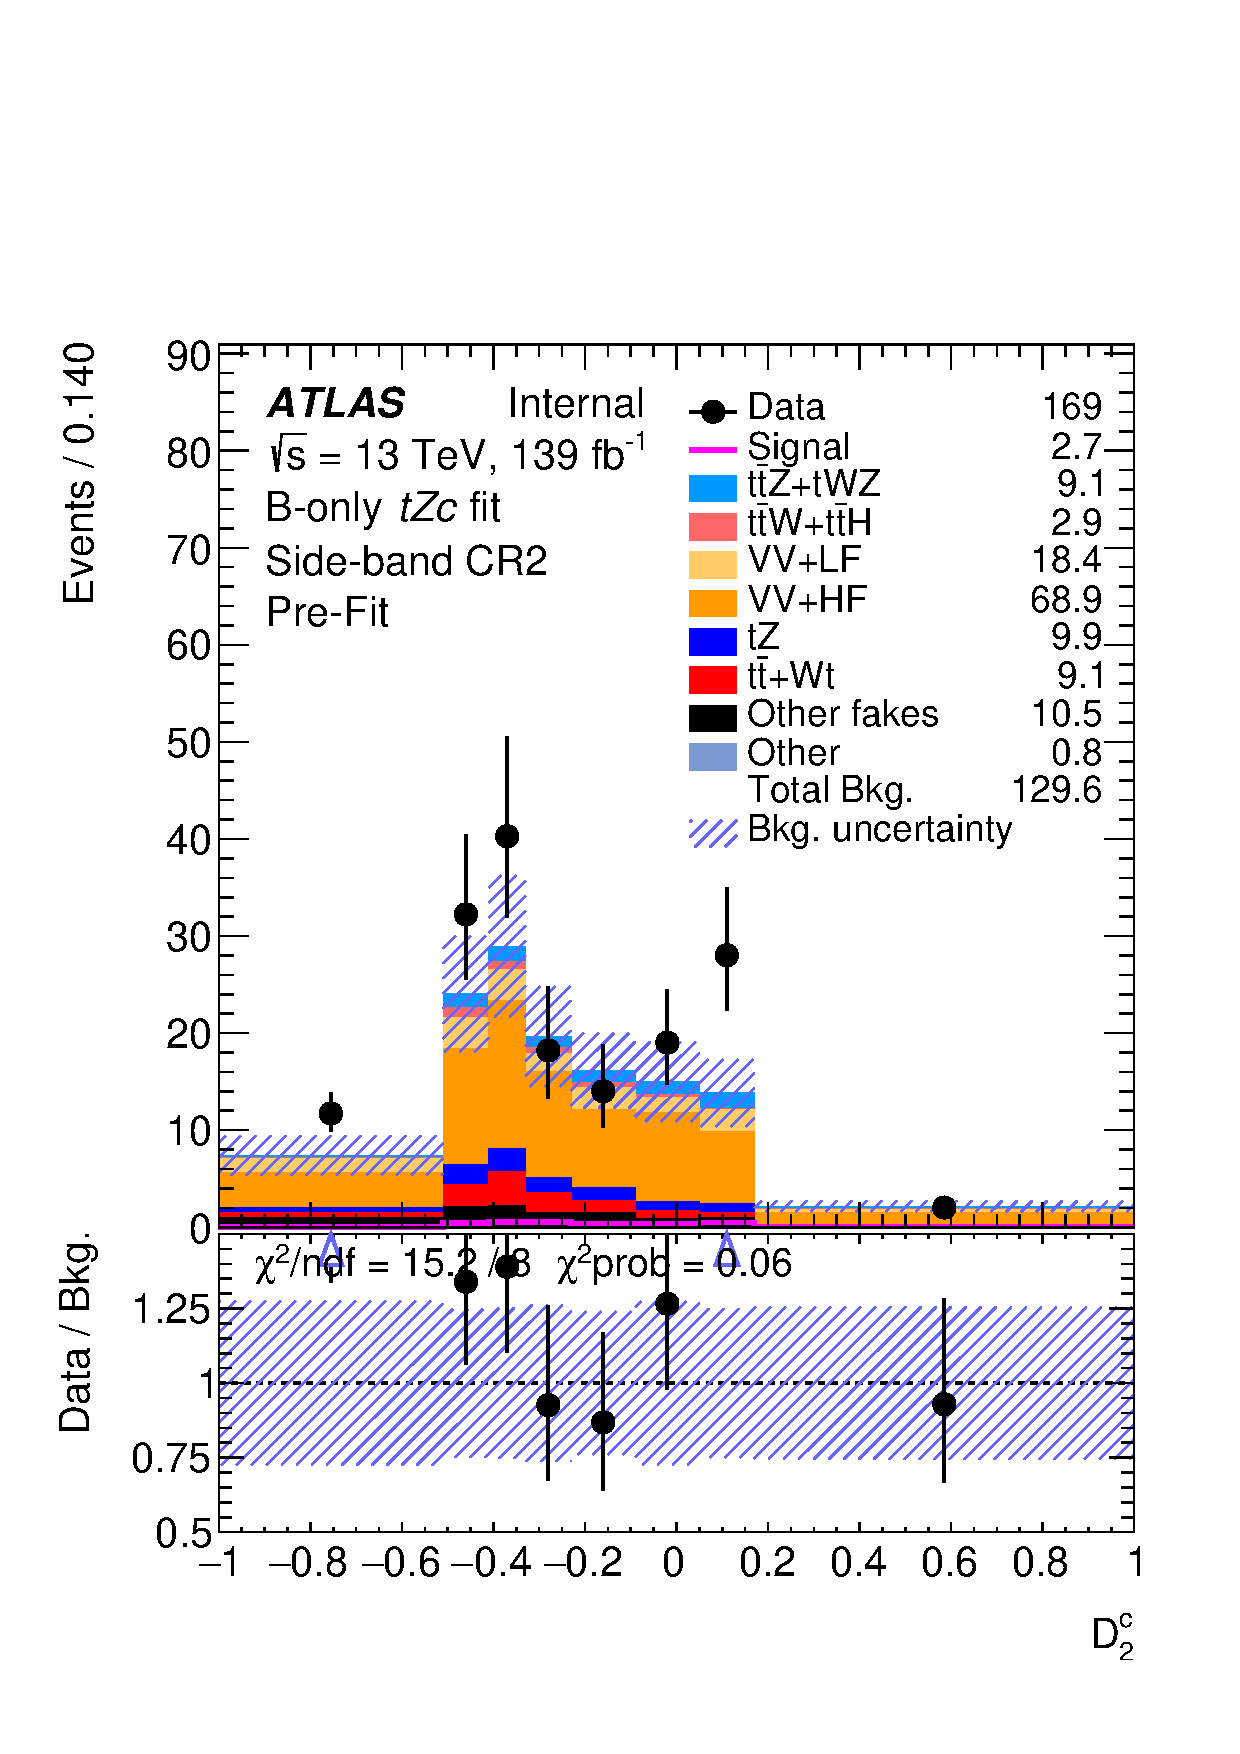
\includegraphics[width=.45\textwidth]{Chapters/CH7/figures/BONLY_CR_UsingDL1rcFullSys/Plots/SBCR2} &
		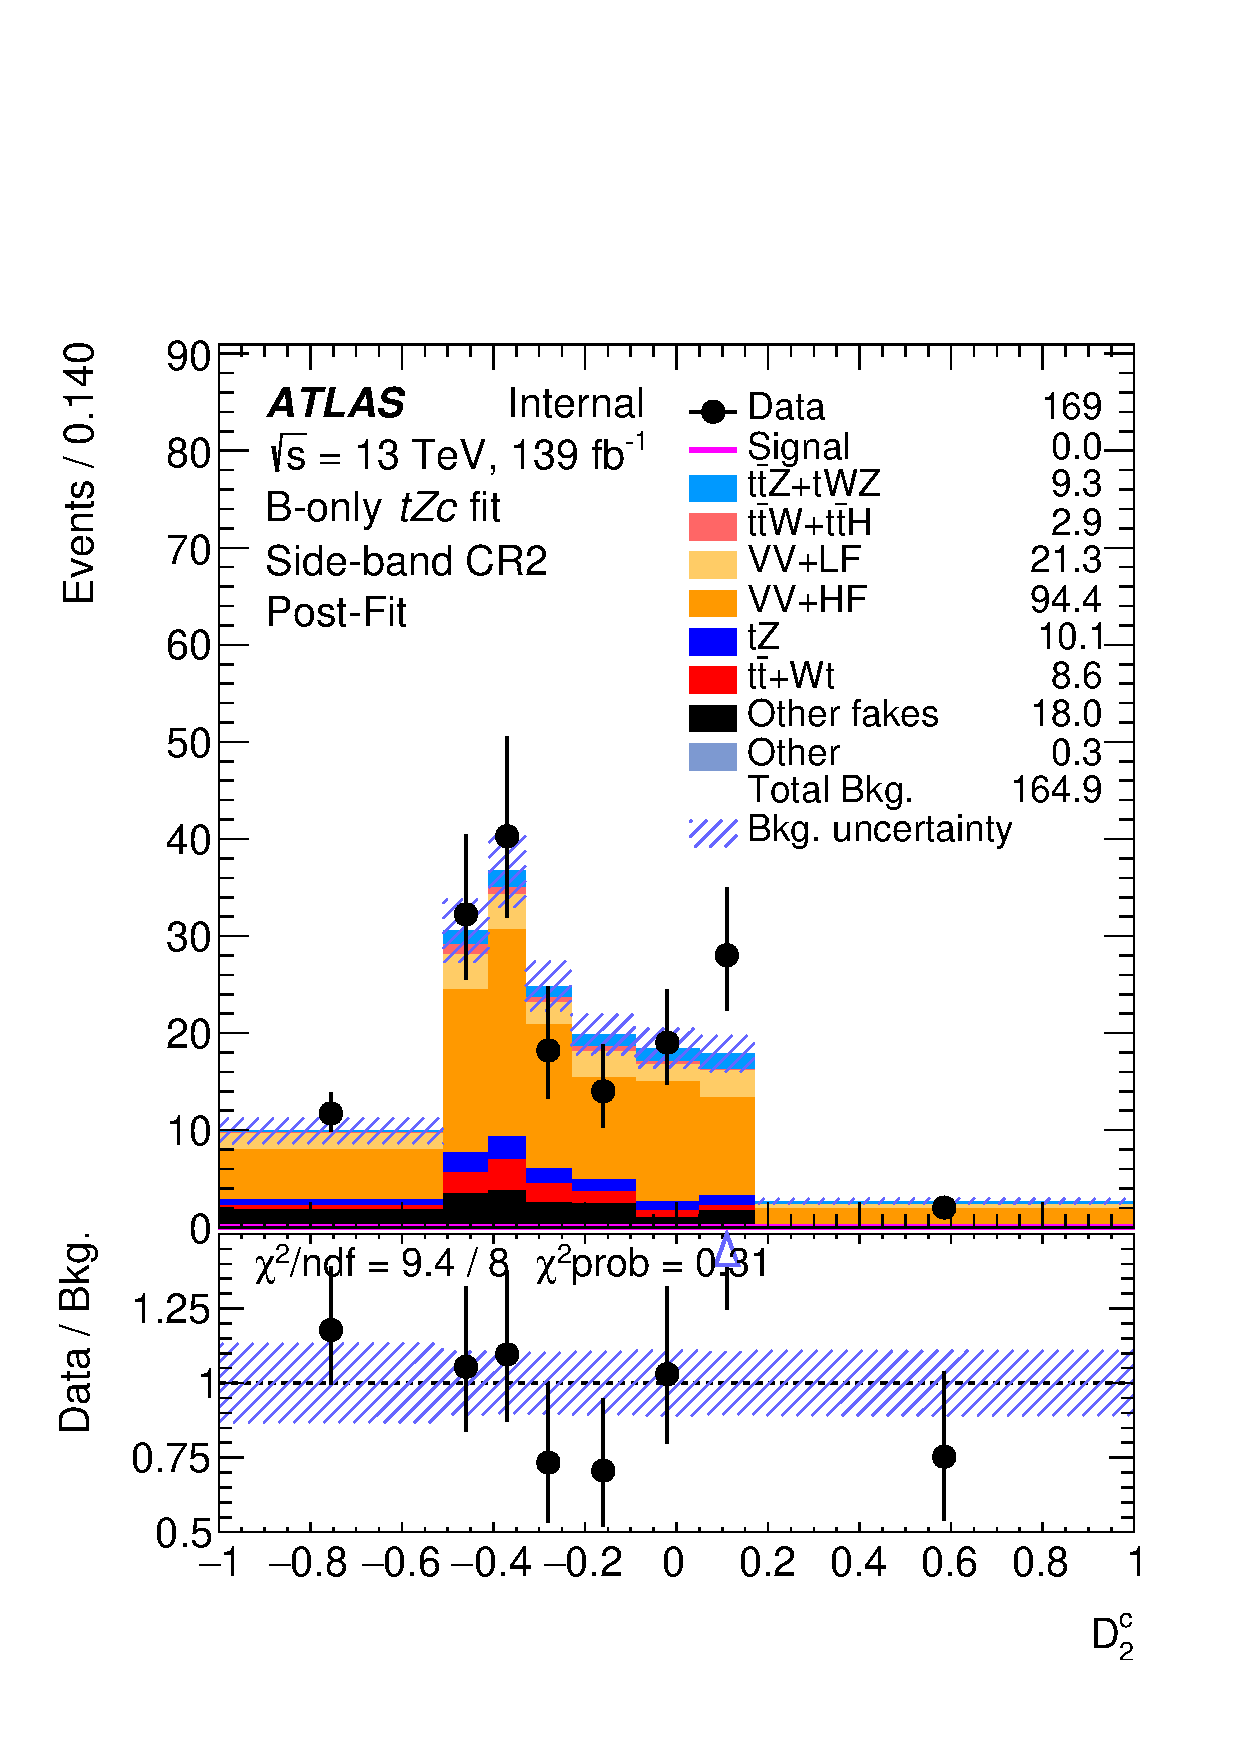
\includegraphics[width=.45\textwidth]{Chapters/CH7/figures/BONLY_CR_UsingDL1rcFullSys/Plots/SBCR2_postFit} \\
	\end{tabular}
	\caption{Pre-fit (left) and post-fit (right) BDTG output distributions in the side-band CRs for the B-only \tZc fit in CRs.
		\ErrStatSys
	}%
	\label{fig:stat:tzc:bonly:cr:crplots:1}
\end{figure}

\begin{figure}[htbp]
	\centering
	\begin{tabular}{cc}
		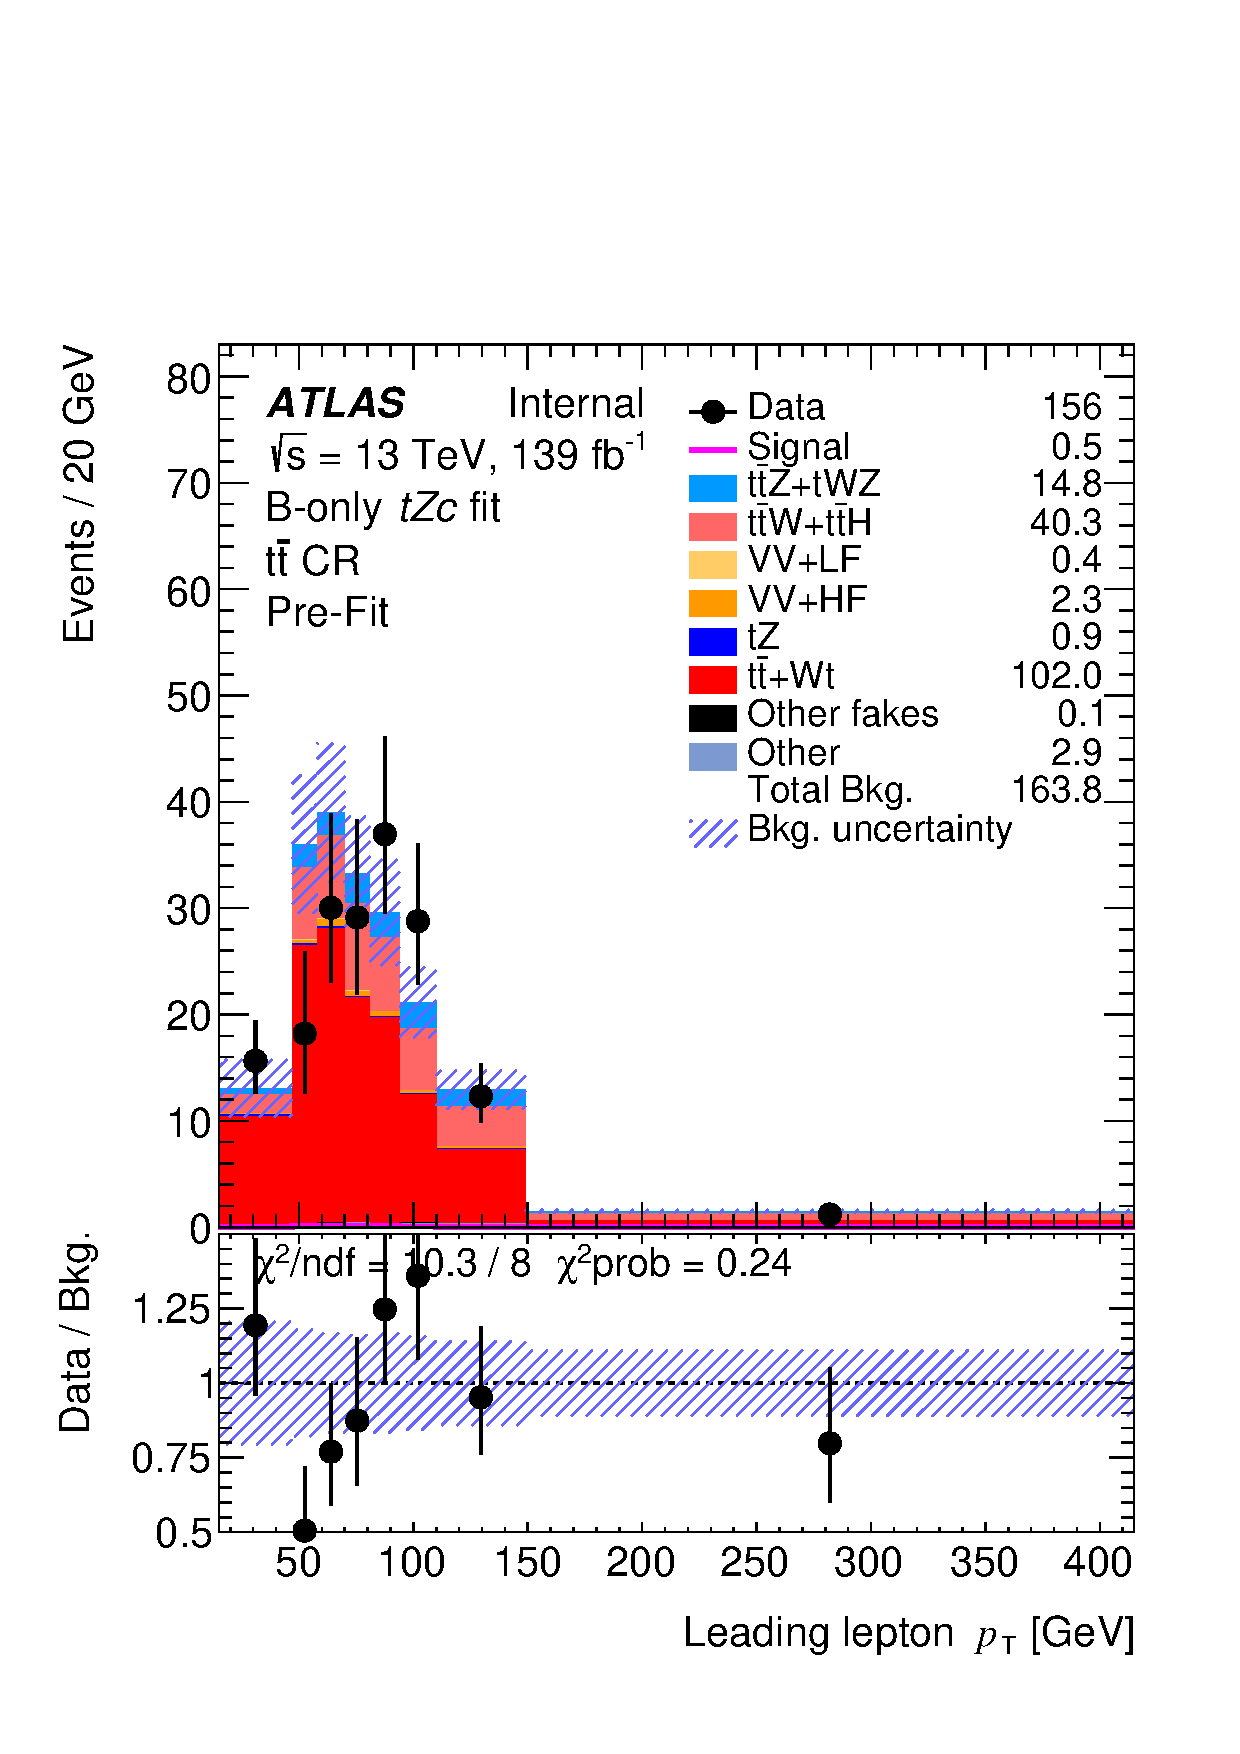
\includegraphics[width=.45\textwidth]{Chapters/CH7/figures/BONLY_CR_UsingDL1rcFullSys/Plots/TTCR} &
		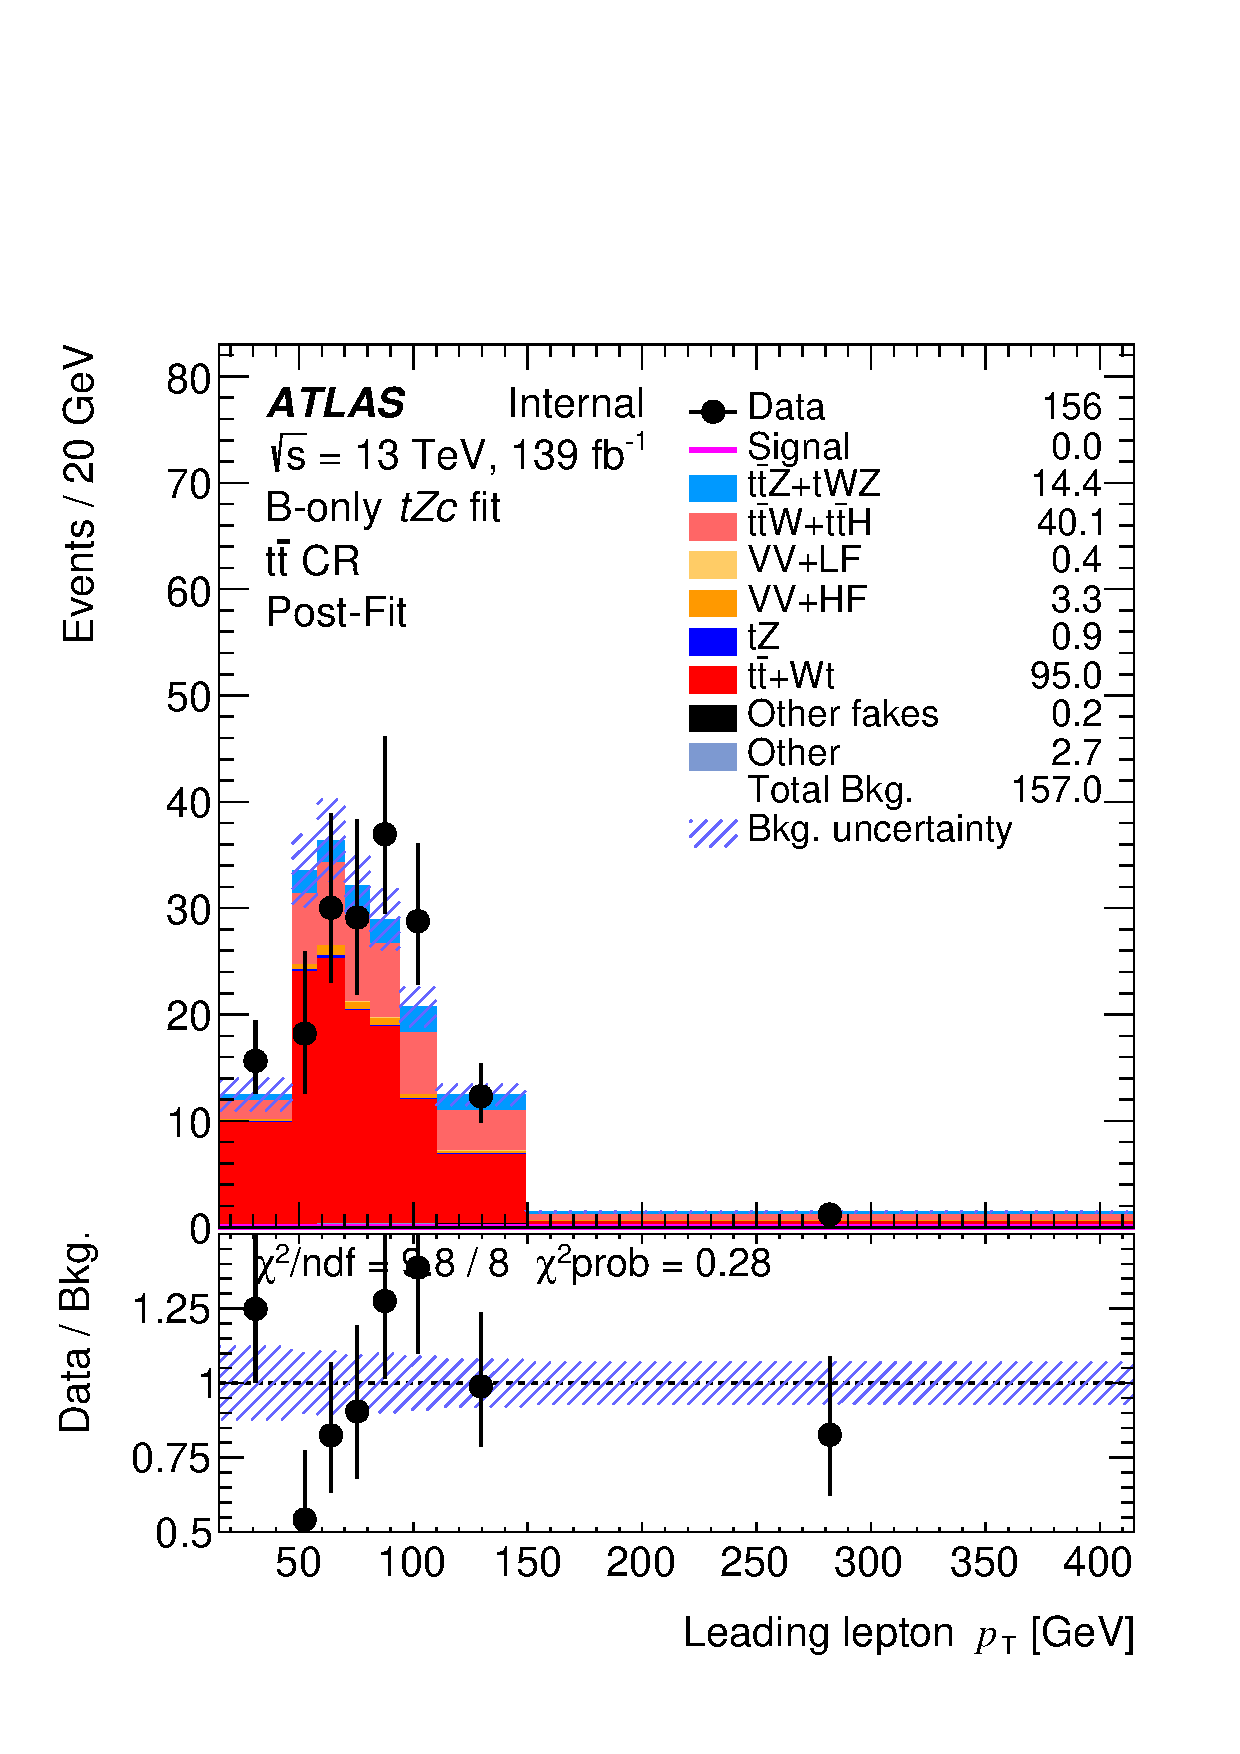
\includegraphics[width=.45\textwidth]{Chapters/CH7/figures/BONLY_CR_UsingDL1rcFullSys/Plots/TTCR_postFit} \\
		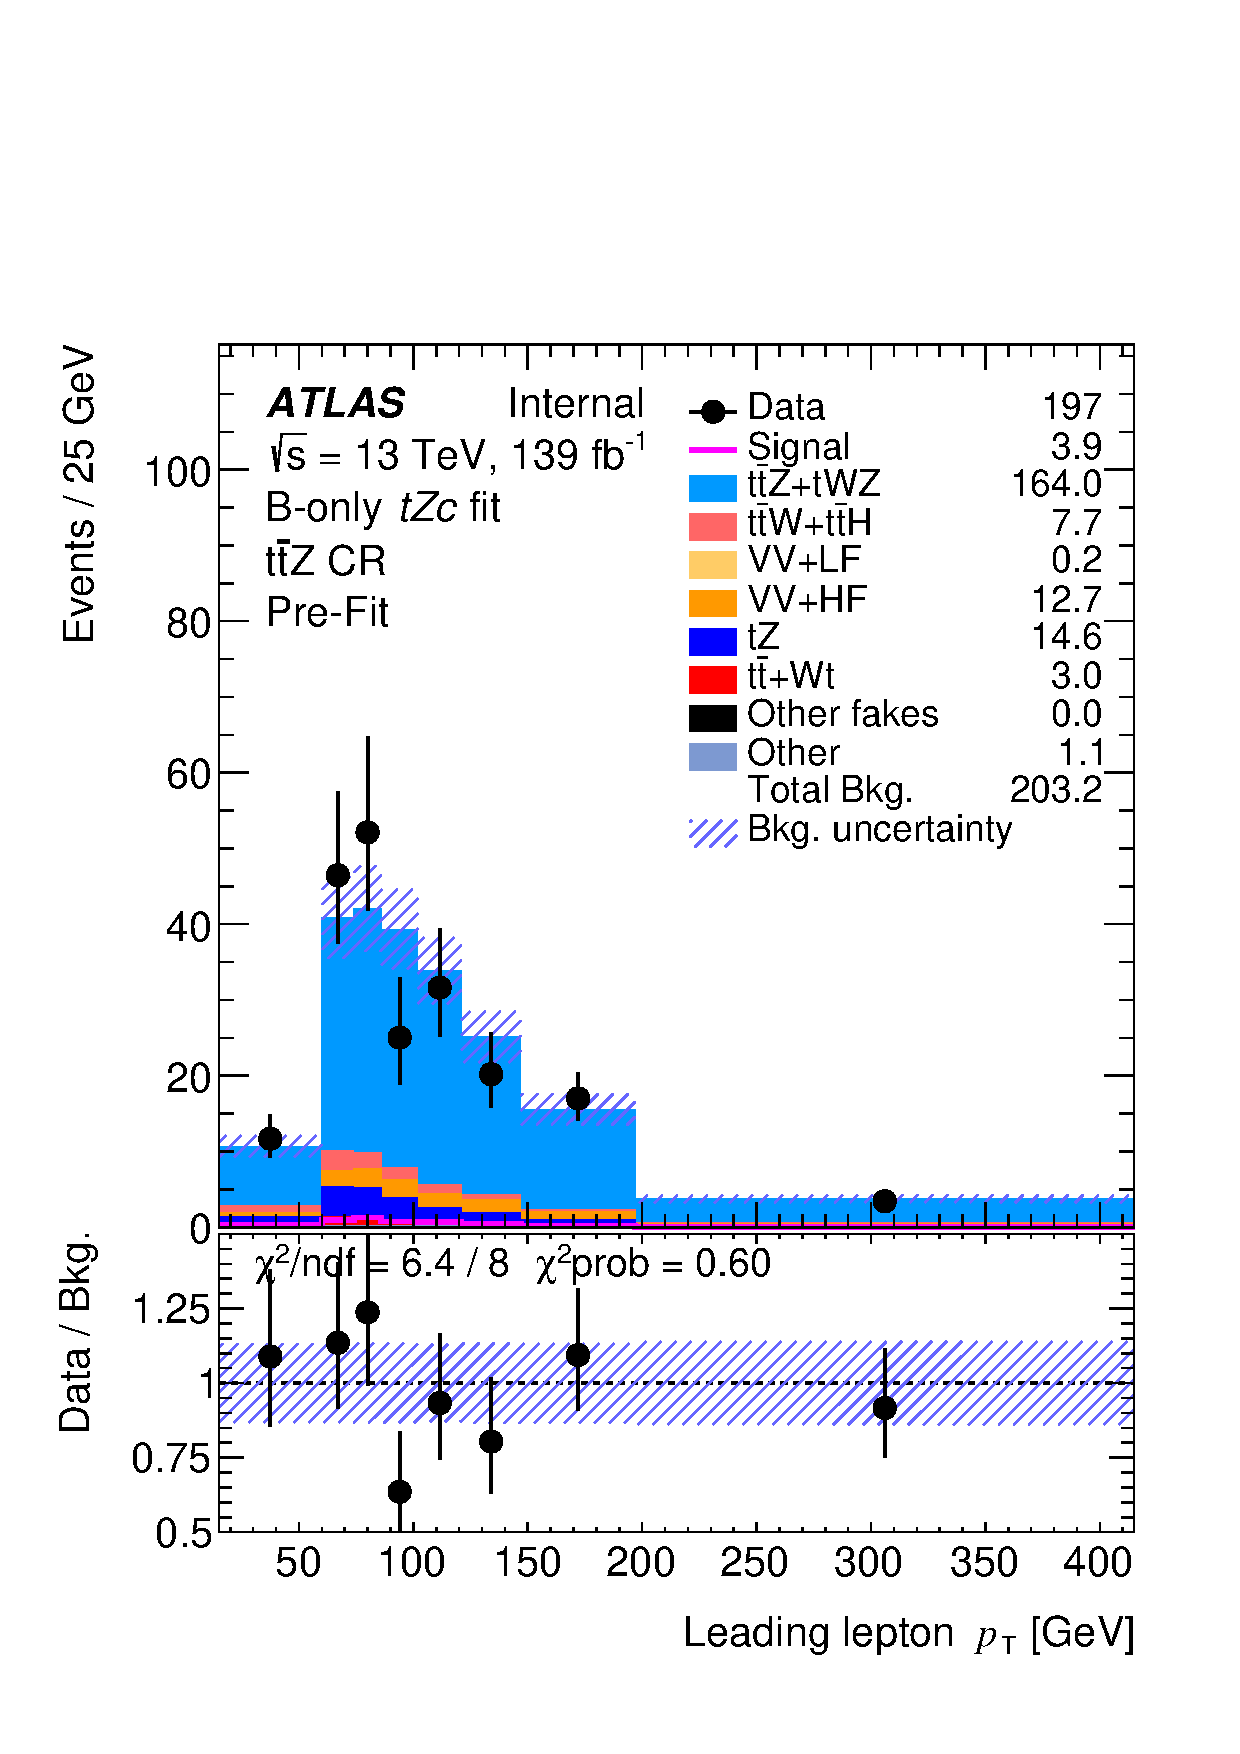
\includegraphics[width=.45\textwidth]{Chapters/CH7/figures/BONLY_CR_UsingDL1rcFullSys/Plots/TTZCR} &
		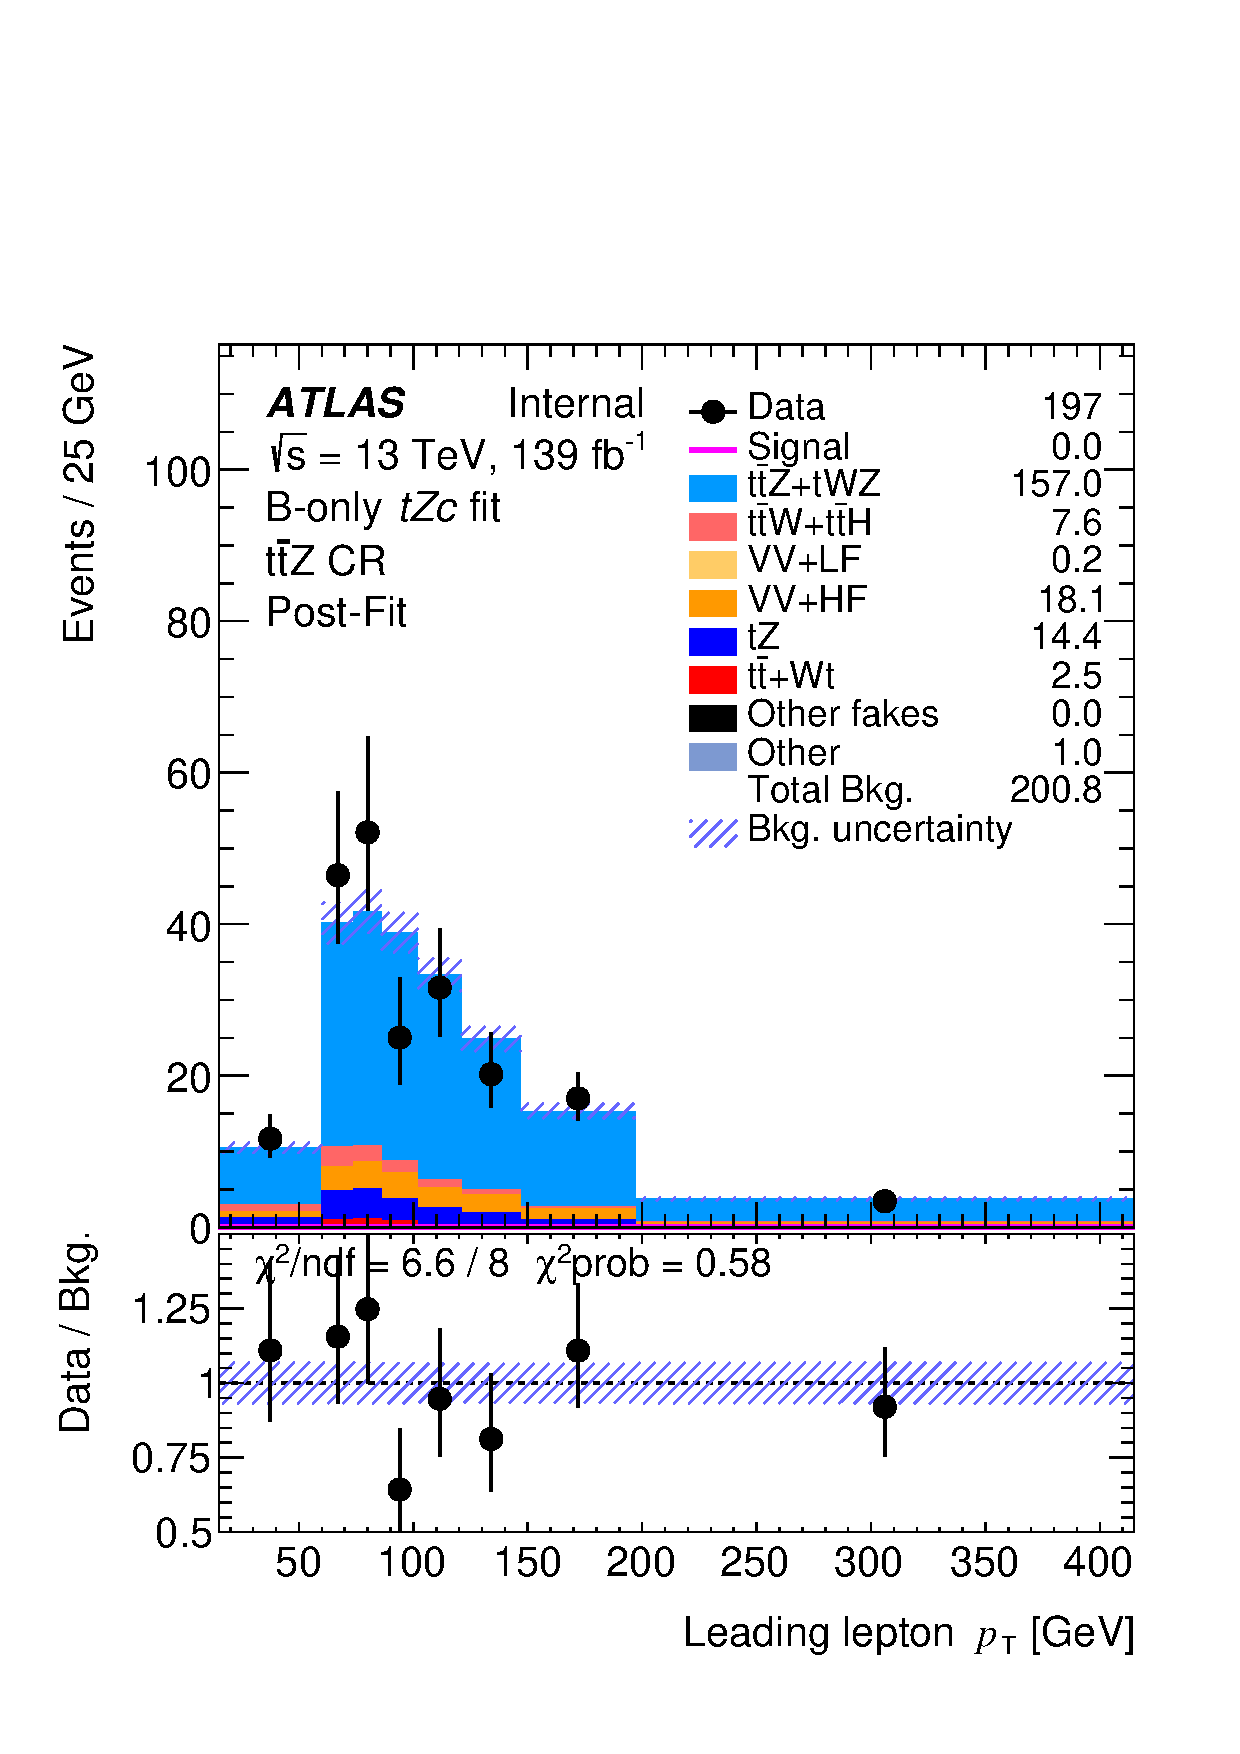
\includegraphics[width=.45\textwidth]{Chapters/CH7/figures/BONLY_CR_UsingDL1rcFullSys/Plots/TTZCR_postFit} \\
	\end{tabular}
	\caption{Pre-fit (left) and post-fit (right) leading lepton \pt distributions in the \ttbar and \ttZ CRs for the B-only \tZc fit in CRs.
		\ErrStatSys
	}%
	\label{fig:stat:tzc:bonly:cr:crplots:2}
\end{figure}
